\chapter{Introduction}
\pagenumbering{arabic}  % 1, 2, 3, 4, ...
\setcounter{page}{1}

Electric energy has become one of the most important source of energy and is widely used resource in world, with ever increasing demand of the (any) resource it becomes more and more difficult to maintain the system and Power System is no exception. Power System has become a complex entity and has gone beyond the limit of manual operattion and control, which makes automation and "smart" control imparitive. This creates demand for new set of measurement, operation and control tools. Out of this tools measurement tools are the most fundamental building block of the modern power system, which is now also know as "smart grid". Measurement devices are "eyes" and "ears" in the system to the centralized "brain", operating-control-corrective system.  

In power system active power and frequency are the most important parameters to be monitored, flow of active power is decided by the phase angle of voltage between buses. Flow of active power decides the structure of network (transmission lines, capacity of devices etc) and hence accurate measurement of it has been of great interest since 1960-70s.\cite{agphadkebook}. Conventionally \textit{relative phase difference} between buses in the network was used, due to limitation of communication links, computational power and the economic pheasibility. This method(s) were slow, moderately accurate and dependent on a tones of heavy and/or manual calcualtion. 
After advancements in telecommunition technology and their speed \& reliability, better computation and satelite availability, trend of \textit{absolute phase difference} measurement came in to existance. The earliest system using absolute phase difference was reported in 1980 using LORAN-C satellite and HBG radio transmission for time reference. And during the same period Global Positioning System was being implemented by US DoD, which was immediately recognised as one of the best way of synchronising the power system, which brought the "Phasor Measurement" and "Synchrophasor" era in to existance. Lot of research was carried out and is being carried out in this area, and flurry of papers are available and are being published in different aspect of synchrophasor measurement. 
\section{Phasors, Synchrophasors and PMUs}
\subsection{Phasors: Defination}

In 1893 C. Steinmetz in his paper introduced simplified mathematcal description of a waveform of an alternating current electricity which he called as "phasor". In Physics and Engineering, \textit{phasor} is a complex number representing a sinusoidal quantity whose amplitude (A), angular velocity ($\omega$) and initial phase ($\phi$) are time-invarient.It is an analytic representation which decomposes sine function in to product of complex constants and a factor which encapsulates the frequency and time dependence. he complex constant, which encapsulates amplitude and phase dependence, is known as phasor, complex amplitude, and (in older texts) sinorx or even complexor.

Which Using Euler's formula can be represented mathematically as:
\begin{equation}\boldmath
Ae^{i(\omega t + \theta)} = A\cos(\omega t + \theta) + A\sin(\omega t + \theta)
\end{equation}

\subsection{Synchronised Phasors or Synchrophasors}
\begin{figure}
	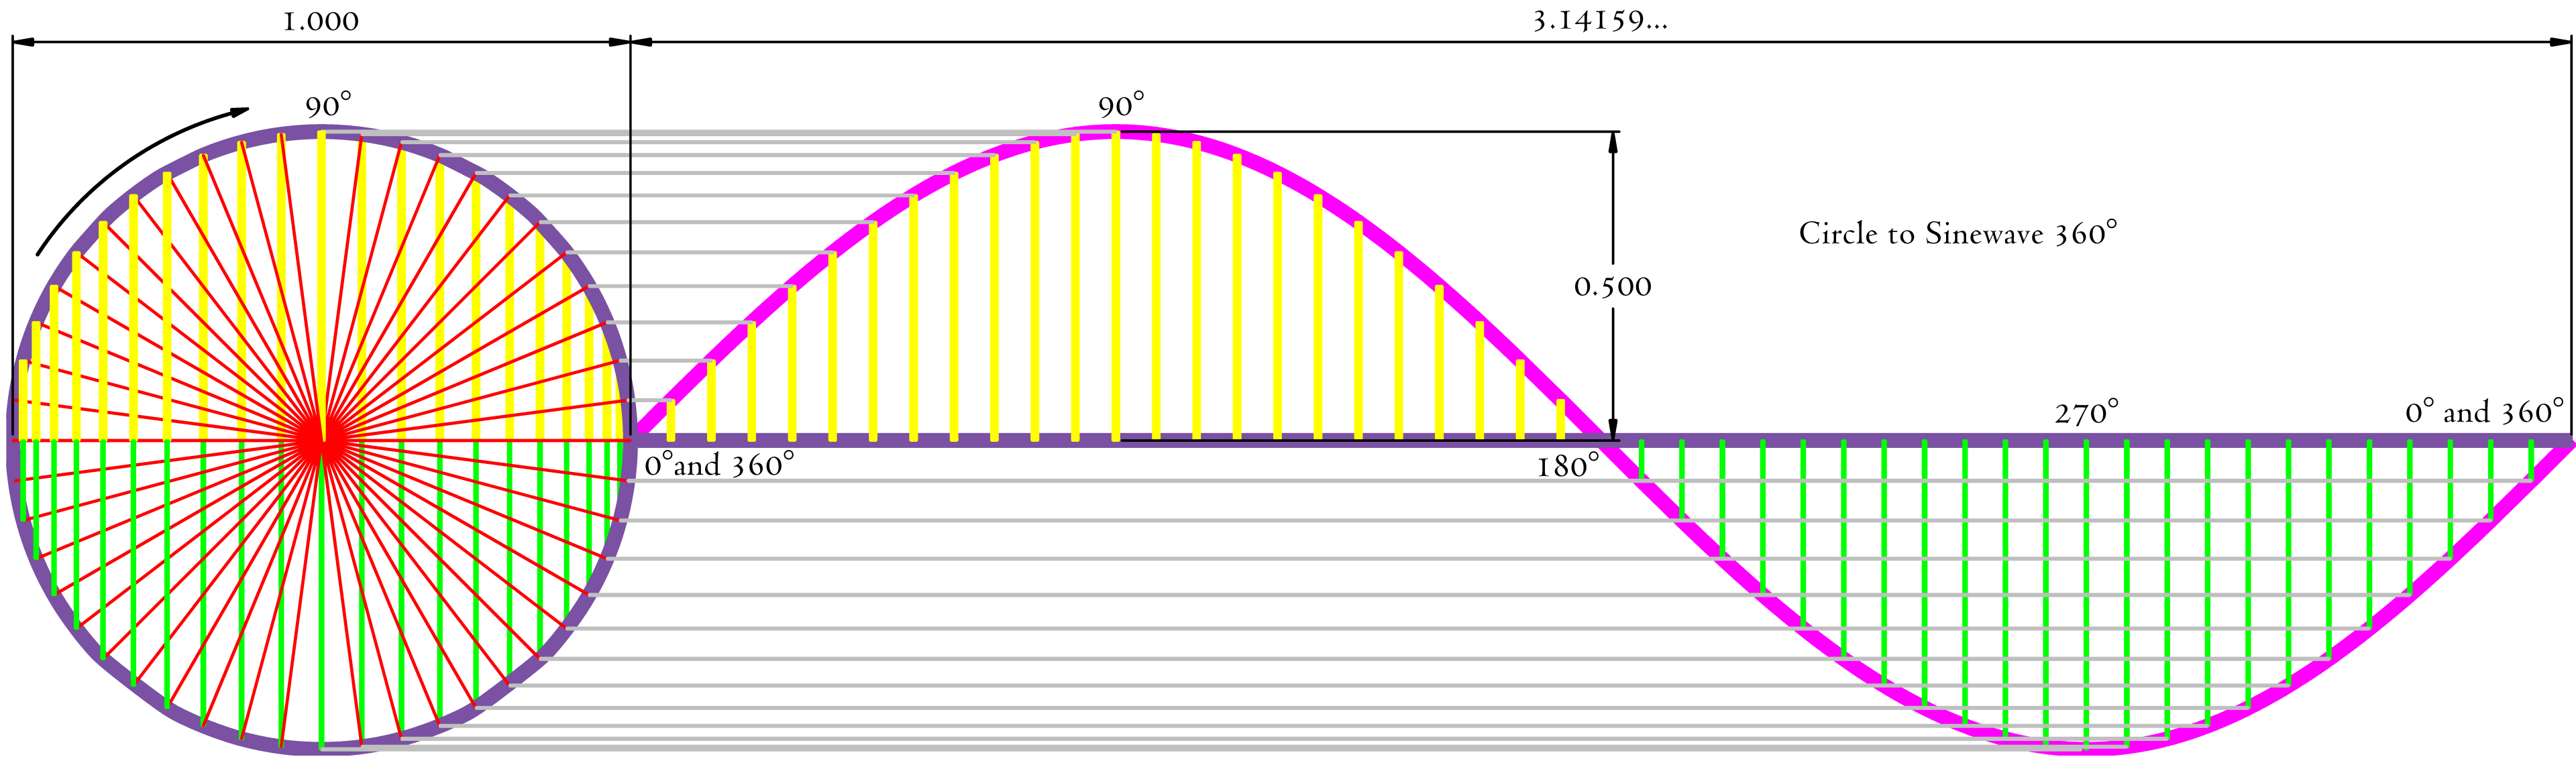
\includegraphics[width=\textwidth]{fig/Circle-To-Sine-Wave.png}
	\caption{Phasor Repsentation, Sampling and synchrophasor \cite{CirSinWave} .} 
	\label{fig:CirSin}
\end{figure}
 Synchronized sampling/measurement of sinusoidal complex quantity (phasor) at a precise reference (time) is called Synchronised Phasor. Time synchronization (of samples) allows synchronized real-time measurements of multiple remote location measurement points on the grid. And this resulting measurement is know as \textbf{synchrophasors} Fig: \ref{fig:CirSin}.
\subsection{Phasor Measurement Unit (PMU)}
PMU is a device which measures and estimates electrical wave in an power network using a common time source for sample synchronization. But it is important to note here that it is an ``estimate" of the phasor(!!) and not the actual measurement. 

This device was first invented by Dr. A. G. Phadke and Dr. James Thorp at Virginia Tech which is considered to be the first sucessful utilization of "phasors" for real-time phasors measurement that were synchronised with accurate absolute time reference provided by GPS.

\section{Wide Area Measurements}

Wide area monitoring systems (WAMS) are essentially based on the new data acquisition technology of phasor measurement and allow monitoring transmission system conditions over large areas in view of detecting and further counteracting grid instabilities. Importance and significance of synchrophasors and PMUs in WAMS can be understood when we see it from the bigger perspective. Consider two geographically distant places like: Kashmir and kaniyakumari or Aasam and Mumbai, How will the phase difference of these two location can be computed? if we want to scale the problem even further we can take American power grid where there exists Time zone difference of 3 Hours ( UTC-8.00 to UTC-5.00 ), how can this be accomplished? This is where PMU and GPS comes into existance, GPS provides an absolute time reference \footnote{\url{http://www.physics.org/article-questions.asp?id=55}} to the PMU which samples the local electrical signal with a global accuracy \footnote{how accurate is GPS? know more \url{http://www.gps.gov/systems/gps/performance/accuracy/}} .